\chapter{Regional Simulations}\label{cha:Regional-Simulations}

%% DK DK got rid of the 2-chunk and 3-chunk options here in the manual (but not in the code) because they are now untested and to my knowledge nobody uses them

The code has the option of running in one-chunk or six-chunk mode.
The one-chunk options may be used for higher resolution regional
simulations. A one-chunk mesh may have lateral dimensions other than
the customary $90^{\circ}$ per chunk, which can further increase
the resolution of the mesh, and thus reduce the shortest period in
the synthetic seismograms (but of course then also reducing the time
step in order for the simulation to remain stable).

A disadvantage of regional simulations is that one needs to use approximate absorbing
boundary conditions on the side and bottom edges of the model (e.g.,
see \citet{KoTr99} for a description of the paraxial boundary conditions
used). Figure~\vref{fig:3D-spectral-element-mesh} and Figure~\vref{fig:Close-up-view-of}
show an example of a one-chunk mesh centered on the Japan subduction
zone, applied in the Japan regional waveform simulation \citep{ChTrHeKa07}.


\section{One-Chunk Simulations}\label{sec:One-Chunk-Simulations}

For a one-chunk regional simulation the following parameters need
to be set in the \texttt{Par\_file}:

\begin{description}
\item [{\texttt{NCHUNKS}}] Must be set to 1.
\item [{\texttt{ANGULAR\_WIDTH\_XI\_IN\_DEGREES}}] Denotes the width of
one side of the chunk ($90^{\circ}$ is a classical value, but you can make it more or less if you want).
\item [{\texttt{ANGULAR\_WIDTH\_ETA\_IN\_DEGREES}}] Denotes the width of
the second side of the chunk ($90^{\circ}$ is a classical value, but you can make it more or less if you want). Note that this
value may be different from \texttt{ANGULAR\_WIDTH\_XI\_IN\_DEGREES}.
\item [{\texttt{CENTER\_LATITUDE\_IN\_DEGREES}}] Defines the latitude of
the center of the chunk (degrees).
\item [{\texttt{CENTER\_LONGITUDE\_IN\_DEGREES}}] Defines the longitude
of the center of the chunk (degrees).
\item [{\texttt{GAMMA\_ROTATION\_AZIMUTH}}] Defines the rotation angle
of the chunk about its center measured counter clockwise from due
North (degrees). The corners of the mesh are output in \texttt{\small OUTPUT\_FILES/values\_from\_mesher.h}.
The output corner progression in \texttt{\small OUTPUT\_FILES/values\_from\_mesher.h}
is bottom left, bottom right, top left, top right. The rotation azimuth
can be changed in the \texttt{Par\_file} and the corners output \texttt{(}\texttt{\small OUTPUT\_FILES/}~\\
\texttt{\small values\_from\_mesher.h}\texttt{)} by using{\small{}
}\texttt{\small xcreate\_header\_file}. It is important to note that
the mesher or the solver does not need to be run to determine the
limits of a 1-chunk simulation.
\item [{\texttt{NEX\_XI}}] The number of spectral elements along the $\xi$ side
of the chunk. This number \textit{must} be 8~$\times$~a multiple
of $\nprocxi$ defined below. For a $90^{\circ}$ chunk, we do not
recommend using $\nexxi$ less than~64 because the curvature of the
Earth cannot be honored if one uses too few elements, which results
in inaccurate and unstable simulations.
\item [{\texttt{NEX\_ETA}}] The number of spectral elements along the $\eta$
side of the chunk. This number \textit{must} be 8~$\times$~a multiple
of $\nproceta$ defined below. Note that in order to get elements
that are close to square on the Earth's surface, the following ratios
should be similar:
\begin{verbatim}
ANGULAR_WIDTH_XI_IN_DEGREES / NEX_XI
ANGULAR_WIDTH_ETA_IN_DEGREES / NEX_ETA
\end{verbatim}
Because of the geometry of the cubed sphere, the option of having
different values for $\nexxi$ and $\nexeta$ is available only for
regional simulations when $\nchunks=1$ (1/6th of the sphere).

\item [{\texttt{NPROC\_XI}}] The number of processors or mesh slices along the
$\xi$ side of the chunk. To accommodate the mesh doubling layers,
we must have $\nexxi=8\times c\times\nprocxi$, where $c\ge1$ is
a positive integer. See Table~\ref{table:nex} for various suitable
choices.
\item [{\texttt{NPROC\_ETA}}] The number of processors or slices along the $\eta$
side of the chunk; we must have $\nexeta=8\times c\times\nproceta$,
where $c\ge1$ is a positive integer. $\nprocxi$ and $\nproceta$
must be equal when $\nchunks=6$.
\end{description}
%
\begin{figure}[H]
\begin{centering}
\includegraphics[scale=0.65]{figures/fig5a.jpg}
\par\end{centering}

\caption{S-wave velocity anomalies
from the global tomographic model s20rts \citep{RiVa00} are superimposed
on the mesh. For parallel computing purposes, the one-chunk SEM simulation
is subdivided in terms of 64 slices. The center of the chunk is at
(38.5$^{\circ}$ N, 137.5$^{\circ}$ E), and the lateral dimensions
are 30$^{\circ}$ $\times$ 30$^{\circ}$. Two doubling layers are
indicated at a depth of 25~km (PREM Moho depth) and a depth of about
1650~km. Shows full view of 25 neighboring slices; see Figure~\ref{fig:Close-up-view-of}
for close-up of upper mantle mesh.}
\label{fig:3D-spectral-element-mesh}
\end{figure}
%
\begin{figure}[H]
\begin{centering}
\includegraphics[scale=0.65]{figures/fig5b.jpg}
\par\end{centering}

\caption{Close-up view of the upper mantle
mesh shown in Figure~\ref{fig:3D-spectral-element-mesh}. Note that
the element size in the crust (top layer) is 13~km $\times$ 13~km,
and that the size of the spectral elements is doubled in the upper
mantle. The velocity variation is captured by NGLL = 5 grid points
in each direction of the elements \citep{KoTr02a,KoTr02b}.}
\label{fig:Close-up-view-of}
\end{figure}


\begin{description}
\item [{\texttt{ABSORBING\_CONDITIONS}}] Set to \texttt{.true.}{\small{}
}for regional simulations. For instance, see \citet{KoTr99} for a
description of the paraxial boundary conditions used. Note that these
conditions are never perfect, and in particular surface waves may
partially reflect off the artificial boundaries. Note also that certain
arrivals, e.g., PKIKPPKIKP, will be missing from the synthetics.
\end{description}
When the width of the chunk is different from $90^{\circ}$ (or the
number of elements is greater than 1248), the radial distribution
of elements needs to be adjusted as well to maintain spectral elements
that are as cube-like as possible. The code attempts to do this, but
be sure to view the mesh with your favorite graphics package to make
sure that the element are well behaved.
Remember: a high-quality mesh is paramount for accurate simulations.
In addition to a reorganization of the radial distribution of elements,
the time stepping and period range in which the attenuation is applied
is automatically determined. The minimum and maximum periods for attenuation
are:

\[
\omega_{max}=\omega_{min}\times10^{W_{3}}\]


\noindent where $W_{3}$ is the optimal width in frequency for 3 Standard
Linear Solids, about 1.75. See \texttt{\small read\_compute\_parameters.f90}
for more details.

The time stepping is determined in a similar fashion as Equation (48)
in \citet{KoTr02a}:

\begin{lyxcode}
dt~=~$S_{c}$~Element~Width~in~km~($r=$ICB)~/~Velocity~($r=$ICB)
\end{lyxcode}
where $S_{c}$ is the stability condition (about 0.4). We use the
radius at the inner core boundary because this is where the maximum
velocity/element width occurs. Again, see \texttt{\small read\_compute\_parameters}\texttt{.f90}
for all the details.

The approximate shortest period at which a regional simulation is
accurate may be determined based upon the relation
\begin{equation}
\mbox{shortest period (s)}\simeq(256/\nexxi)\times(\texttt{ANGULAR\_WIDTH\_XI\_IN\_DEGREES}/90)\times17.\label{eq:shortest_period_regional}\end{equation}



% \section{Two-Chunk Simulations}
%
% For a two-chunk regional simulation the following parameters need
% to be set in the \texttt{Par\_file}:
%
% \begin{description}
% \item [{$\nchunks$}] Must be set to 2
% \item [{\texttt{ANGULAR\_WIDTH\_XI\_IN\_DEGREES}}] Denotes the width of
% one side of the chunk, and it has to be 90 degrees.
% \item [{\texttt{ANGULAR\_WIDTH\_ETA\_IN\_DEGREES}}] Denotes the width of
% the second side of the chunk, and it also has to be 90 degrees.
% \end{description}
% \texttt{NEX\_XI} and \texttt{NEX\_ETA} follow the same description
% in Section \ref{sec:One-Chunk-Simulations}, however, they need to
% be the same in this case. All other parameters are similar to the
% one-chunk simulations, refer to Section \ref{sec:One-Chunk-Simulations}
% for details.
%
% %
% \begin{figure}[H]
% \noindent \begin{centering}
% 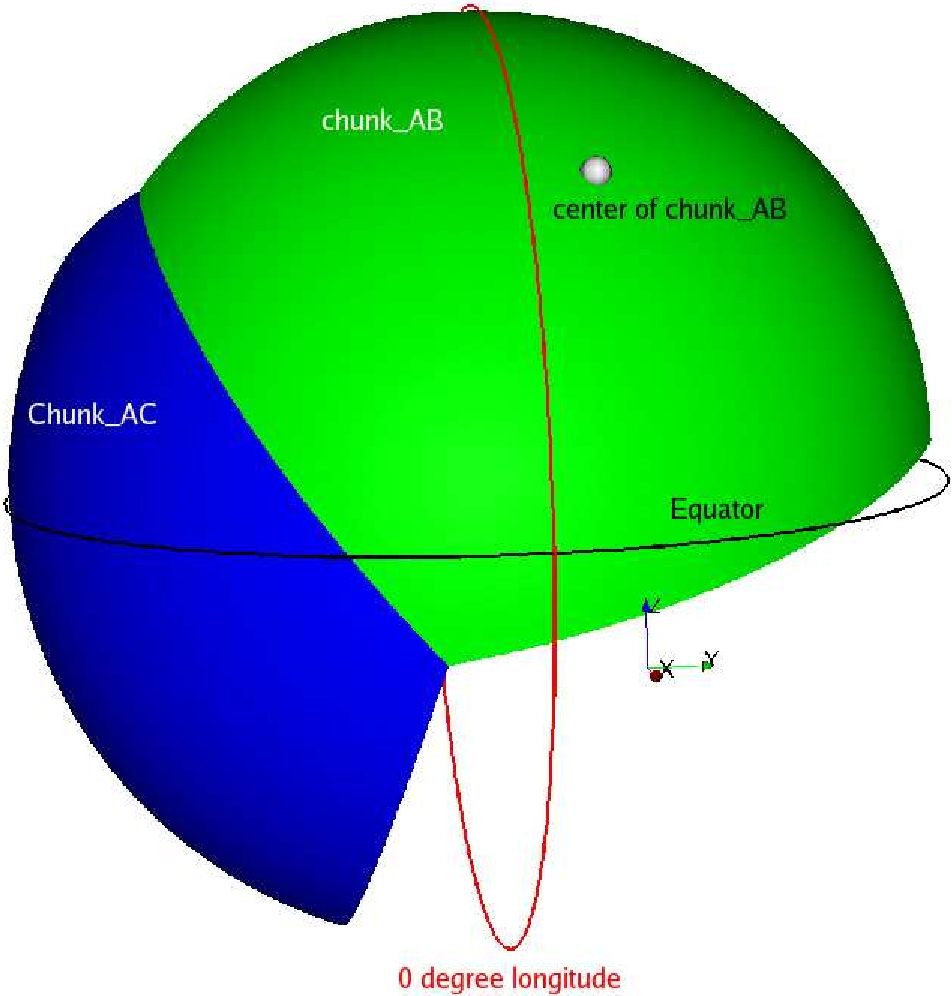
\includegraphics[width=0.6\textwidth]{figures/2-chunk-surface}
% \par\end{centering}
%
% \caption{Geometry of a 2-chunk simulation, where the first chunk (\texttt{CHUNK\_AB})
% centers at $40^{\circ}$ latitude, $10^{\circ}$ longitude, and has
% been rotated by $20^{\circ}$ counter clockwise, and the second chunk
% (\texttt{CHUNK\_AC}) connects to the first chunk through one face.}
%
% \end{figure}




